\documentclass[14pt]{extbook}
\usepackage{multicol, enumerate, enumitem, hyperref, color, soul, setspace, parskip, fancyhdr} %General Packages
\usepackage{amssymb, amsthm, amsmath, bbm, latexsym, units, mathtools} %Math Packages
\everymath{\displaystyle} %All math in Display Style
% Packages with additional options
\usepackage[headsep=0.5cm,headheight=12pt, left=1 in,right= 1 in,top= 1 in,bottom= 1 in]{geometry}
\usepackage[usenames,dvipsnames]{xcolor}
\usepackage{dashrule}  % Package to use the command below to create lines between items
\newcommand{\litem}[1]{\item#1\hspace*{-1cm}\rule{\textwidth}{0.4pt}}
\pagestyle{fancy}
\lhead{Progress Quiz 4}
\chead{}
\rhead{Version C}
\lfoot{6286-1986}
\cfoot{}
\rfoot{Fall 2020}
\begin{document}

\begin{enumerate}
\litem{
Factor the quadratic below. Then, choose the intervals that contain the constants in the form $(ax+b)(cx+d); b \leq d.$\[ 24x^{2} -10 x -25 \]\begin{enumerate}[label=\Alph*.]
\item \( a \in [-1, 2], \hspace*{5mm} b \in [-5, 0], \hspace*{5mm} c \in [16.4, 18.8], \text{ and } \hspace*{5mm} d \in [1, 7] \)
\item \( a \in [8, 9], \hspace*{5mm} b \in [-5, 0], \hspace*{5mm} c \in [1.5, 3.8], \text{ and } \hspace*{5mm} d \in [1, 7] \)
\item \( a \in [4, 6], \hspace*{5mm} b \in [-5, 0], \hspace*{5mm} c \in [3.8, 9.9], \text{ and } \hspace*{5mm} d \in [1, 7] \)
\item \( a \in [-1, 2], \hspace*{5mm} b \in [-33, -26], \hspace*{5mm} c \in [0.7, 2.9], \text{ and } \hspace*{5mm} d \in [14, 22] \)
\item \( \text{None of the above.} \)

\end{enumerate} }
\litem{
Solve the quadratic equation below. Then, choose the intervals that the solutions belong to, with $x_1 \leq x_2$ (if they exist).\[ -16x^{2} -8 x + 6 = 0 \]\begin{enumerate}[label=\Alph*.]
\item \( x_1 \in [-7.6, -6.4] \text{ and } x_2 \in [14.29, 15] \)
\item \( x_1 \in [-0.6, 0] \text{ and } x_2 \in [0.52, 1.93] \)
\item \( x_1 \in [-23.3, -20.3] \text{ and } x_2 \in [20.09, 21.84] \)
\item \( x_1 \in [-1.1, -0.5] \text{ and } x_2 \in [-0.08, 0.72] \)
\item \( \text{There are no Real solutions.} \)

\end{enumerate} }
\litem{
Write the equation of the graph presented below in the form $f(x)=ax^2+bx+c$, assuming  $a=1$ or $a=-1$. Then, choose the intervals that $a, b,$ and $c$ belong to.
\begin{center}
    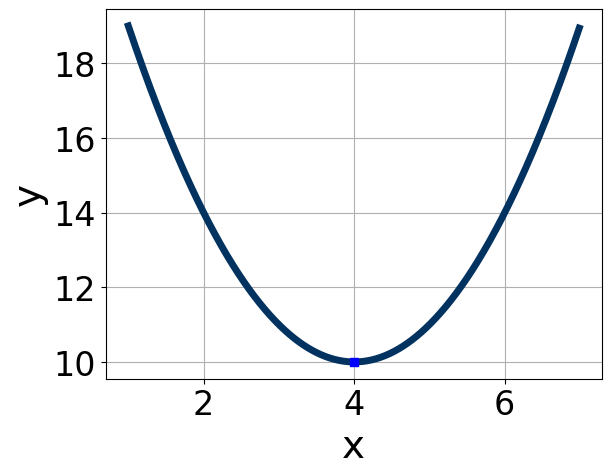
\includegraphics[width=0.5\textwidth]{../Figures/quadraticGraphToEquationC.png}
\end{center}
\begin{enumerate}[label=\Alph*.]
\item \( a \in [0, 4], \hspace*{5mm} b \in [7, 11], \text{ and } \hspace*{5mm} c \in [19, 29] \)
\item \( a \in [-1, 0], \hspace*{5mm} b \in [7, 11], \text{ and } \hspace*{5mm} c \in [-10, -9] \)
\item \( a \in [-1, 0], \hspace*{5mm} b \in [-9, -5], \text{ and } \hspace*{5mm} c \in [-10, -9] \)
\item \( a \in [0, 4], \hspace*{5mm} b \in [-9, -5], \text{ and } \hspace*{5mm} c \in [9, 12] \)
\item \( a \in [0, 4], \hspace*{5mm} b \in [-9, -5], \text{ and } \hspace*{5mm} c \in [19, 29] \)

\end{enumerate} }
\litem{
Graph the equation below.\[ f(x) = -(x+1)^2 + 14 \]\begin{enumerate}[label=\Alph*.]
\begin{multicols}{2}\item 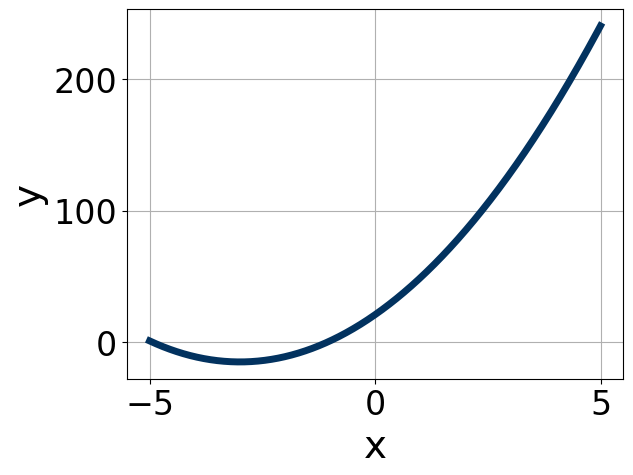
\includegraphics[width = 0.3\textwidth]{../Figures/quadraticEquationToGraphAC.png}\item 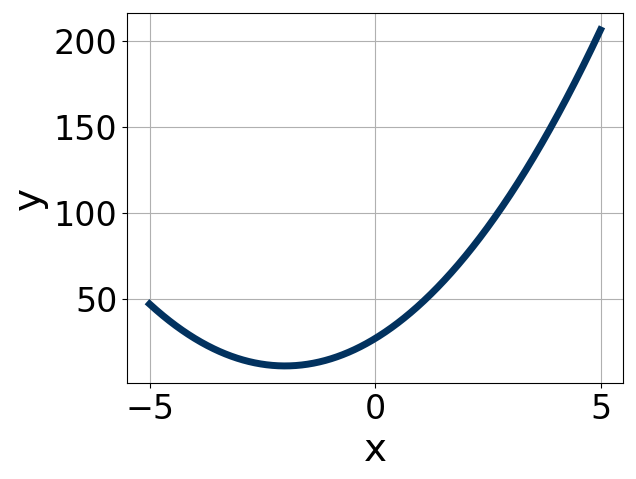
\includegraphics[width = 0.3\textwidth]{../Figures/quadraticEquationToGraphBC.png}\item 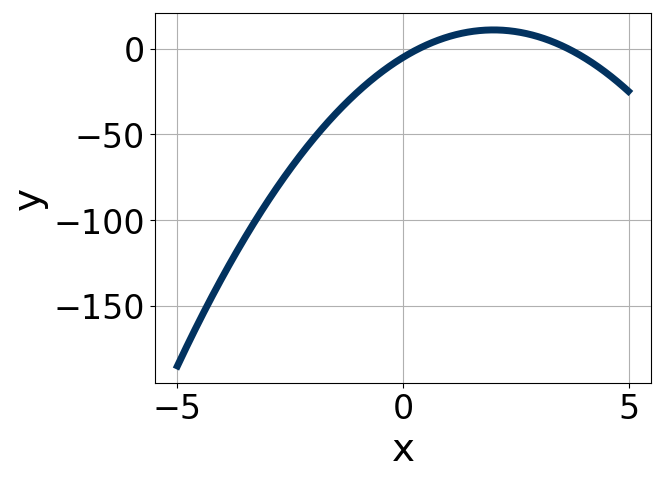
\includegraphics[width = 0.3\textwidth]{../Figures/quadraticEquationToGraphCC.png}\item 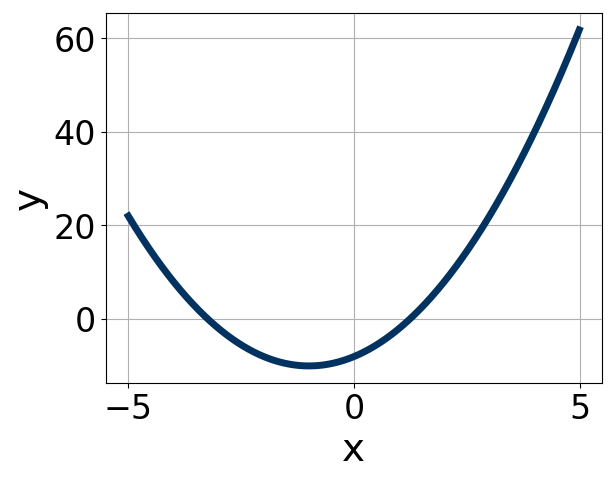
\includegraphics[width = 0.3\textwidth]{../Figures/quadraticEquationToGraphDC.png}\end{multicols}\item None of the above.
\end{enumerate} }
\litem{
Write the equation of the graph presented below in the form $f(x)=ax^2+bx+c$, assuming  $a=1$ or $a=-1$. Then, choose the intervals that $a, b,$ and $c$ belong to.
\begin{center}
    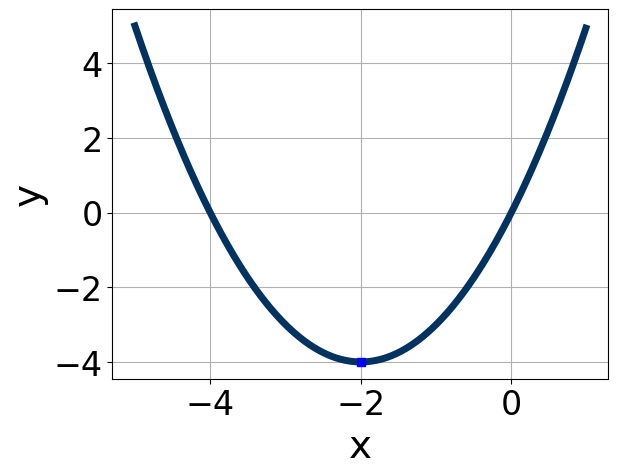
\includegraphics[width=0.5\textwidth]{../Figures/quadraticGraphToEquationCopyC.png}
\end{center}
\begin{enumerate}[label=\Alph*.]
\item \( a \in [0.4, 2.4], \hspace*{5mm} b \in [6, 10], \text{ and } \hspace*{5mm} c \in [16, 21] \)
\item \( a \in [-2.1, -0.2], \hspace*{5mm} b \in [-8, -2], \text{ and } \hspace*{5mm} c \in [-15, -13] \)
\item \( a \in [0.4, 2.4], \hspace*{5mm} b \in [-8, -2], \text{ and } \hspace*{5mm} c \in [10, 16] \)
\item \( a \in [0.4, 2.4], \hspace*{5mm} b \in [-8, -2], \text{ and } \hspace*{5mm} c \in [16, 21] \)
\item \( a \in [-2.1, -0.2], \hspace*{5mm} b \in [6, 10], \text{ and } \hspace*{5mm} c \in [-15, -13] \)

\end{enumerate} }
\litem{
Graph the equation below.\[ f(x) = (x+2)^2 + 14 \]\begin{enumerate}[label=\Alph*.]
\begin{multicols}{2}\item 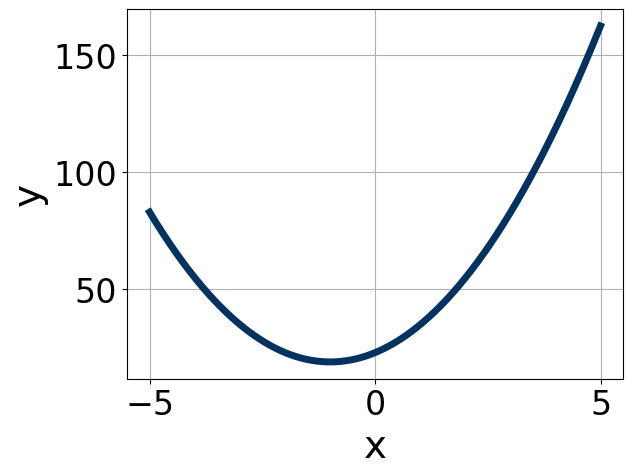
\includegraphics[width = 0.3\textwidth]{../Figures/quadraticEquationToGraphCopyAC.png}\item 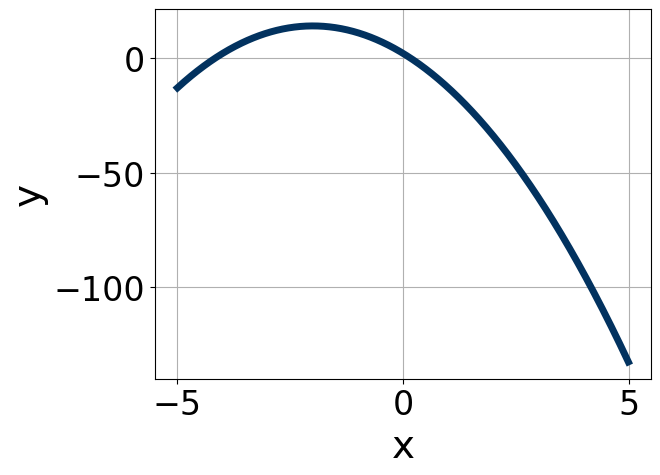
\includegraphics[width = 0.3\textwidth]{../Figures/quadraticEquationToGraphCopyBC.png}\item 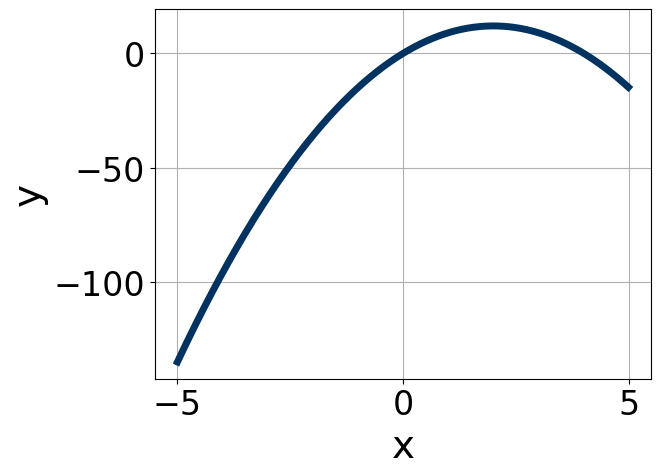
\includegraphics[width = 0.3\textwidth]{../Figures/quadraticEquationToGraphCopyCC.png}\item 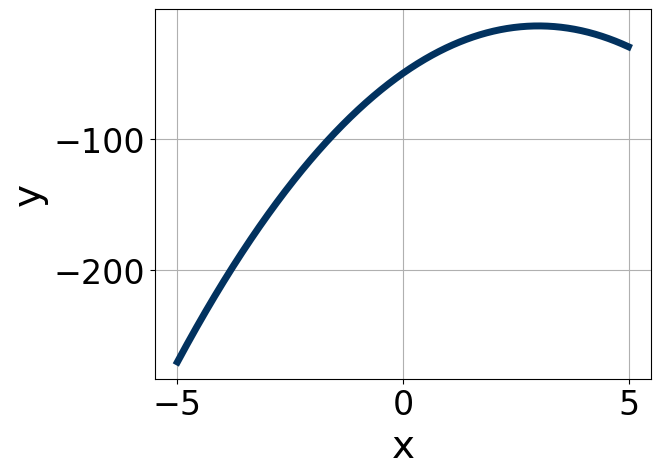
\includegraphics[width = 0.3\textwidth]{../Figures/quadraticEquationToGraphCopyDC.png}\end{multicols}\item None of the above.
\end{enumerate} }
\litem{
Factor the quadratic below. Then, choose the intervals that contain the constants in the form $(ax+b)(cx+d); b \leq d.$\[ 16x^{2} -32 x + 15 \]\begin{enumerate}[label=\Alph*.]
\item \( a \in [3.64, 4.23], \hspace*{5mm} b \in [-9, -3], \hspace*{5mm} c \in [2.57, 4.27], \text{ and } \hspace*{5mm} d \in [-6, 2] \)
\item \( a \in [-0.01, 1.45], \hspace*{5mm} b \in [-25, -18], \hspace*{5mm} c \in [-0.12, 1.03], \text{ and } \hspace*{5mm} d \in [-12, -8] \)
\item \( a \in [1.5, 3.59], \hspace*{5mm} b \in [-9, -3], \hspace*{5mm} c \in [7.18, 8.42], \text{ and } \hspace*{5mm} d \in [-6, 2] \)
\item \( a \in [7.55, 8.16], \hspace*{5mm} b \in [-9, -3], \hspace*{5mm} c \in [1.96, 2.26], \text{ and } \hspace*{5mm} d \in [-6, 2] \)
\item \( \text{None of the above.} \)

\end{enumerate} }
\litem{
Solve the quadratic equation below. Then, choose the intervals that the solutions $x_1$ and $x_2$ belong to, with $x_1 \leq x_2$.\[ 10x^{2} -33 x -54 = 0 \]\begin{enumerate}[label=\Alph*.]
\item \( x_1 \in [-1.3, -1.1] \text{ and } x_2 \in [3.97, 5.26] \)
\item \( x_1 \in [-9.8, -4.1] \text{ and } x_2 \in [0.86, 1.41] \)
\item \( x_1 \in [-12.3, -11.7] \text{ and } x_2 \in [44.45, 45.17] \)
\item \( x_1 \in [-4.7, -1.3] \text{ and } x_2 \in [1.16, 2.62] \)
\item \( x_1 \in [-0.8, 0.9] \text{ and } x_2 \in [13.03, 14.14] \)

\end{enumerate} }
\litem{
Solve the quadratic equation below. Then, choose the intervals that the solutions belong to, with $x_1 \leq x_2$ (if they exist).\[ 13x^{2} -14 x -4 = 0 \]\begin{enumerate}[label=\Alph*.]
\item \( x_1 \in [-1.7, -0.4] \text{ and } x_2 \in [0.1, 1.2] \)
\item \( x_1 \in [-20.3, -19] \text{ and } x_2 \in [19.4, 22.9] \)
\item \( x_1 \in [-4.7, -2.2] \text{ and } x_2 \in [16.9, 19.7] \)
\item \( x_1 \in [-1.1, 0.8] \text{ and } x_2 \in [1.2, 1.9] \)
\item \( \text{There are no Real solutions.} \)

\end{enumerate} }
\litem{
Solve the quadratic equation below. Then, choose the intervals that the solutions $x_1$ and $x_2$ belong to, with $x_1 \leq x_2$.\[ 10x^{2} +33 x -54 = 0 \]\begin{enumerate}[label=\Alph*.]
\item \( x_1 \in [-9.1, -6.7] \text{ and } x_2 \in [0.41, 1.11] \)
\item \( x_1 \in [-4.2, -1.2] \text{ and } x_2 \in [2.22, 2.72] \)
\item \( x_1 \in [-6.4, -3] \text{ and } x_2 \in [0.74, 1.25] \)
\item \( x_1 \in [-45.2, -44.5] \text{ and } x_2 \in [11.86, 12.02] \)
\item \( x_1 \in [-14.1, -11.7] \text{ and } x_2 \in [0.22, 0.47] \)

\end{enumerate} }
\end{enumerate}

\end{document}